\documentclass[aspectratio=169]{beamer}
\usetheme{Madrid}
\usecolortheme{seahorse}
\setbeamertemplate{navigation symbols}{}
\setbeamertemplate{footline}[frame number]
\setbeamersize{text margin left=8mm,text margin right=8mm}

\usepackage{amsmath,amssymb,bm}
\usepackage{braket}
\usepackage{booktabs}
\usepackage{graphicx}
\graphicspath{{./asset/}{./assets/}}
\usepackage{tikz}
\usetikzlibrary{arrows.meta,positioning,calc}
\setlength{\abovedisplayskip}{5pt}
\setlength{\belowdisplayskip}{5pt}

\title{MNIST Training with DQNN/IDQNN}
\author{}
\institute{Quantum Machine Learning}
\date{\today}

\begin{document}

\begin{frame}
  \maketitle
\end{frame}

% \begin{frame}{Outline}
%   \begin{itemize}
%     \item Algorithm recap: inference and learning
%     \item MNIST task definition and preprocessing
%     \item Label encoding and training details
%     \item Efficiency and generation results
%     \item Conclusions
%   \end{itemize}
% \end{frame}


\section{Algorithm Recap}

\begin{frame}{Generate bitstring with DQNN/IDQNN}
  % \begin{block}{Inference stage}
  %   Given an input bitstring $x\in\{0,1\}^n$, the generative quantum model produces output bitstring $y\in\{0,1\}^n$ with parameters $\theta$:
  %   \[
  %     y \sim p_\theta(y\mid x).
  %   \]
  % \end{block}

  {\centering
  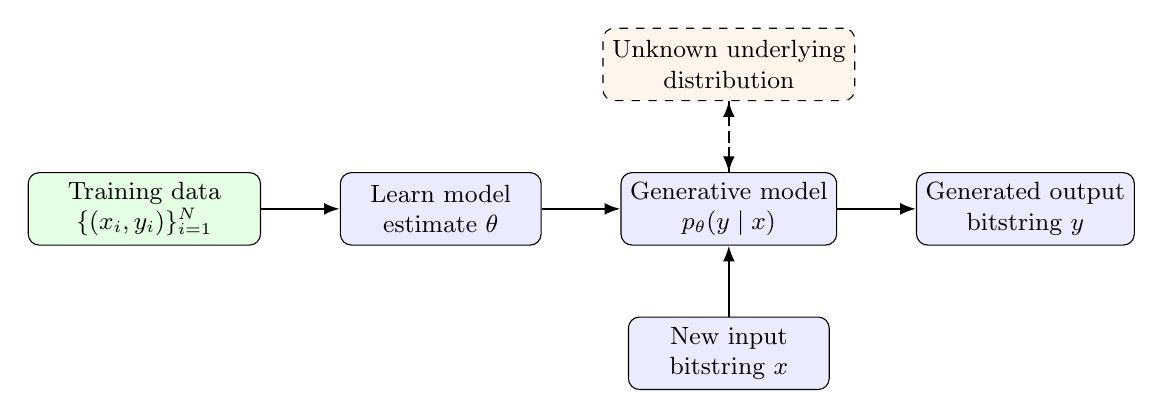
\begin{tikzpicture}[
    font=\small,
    node distance=8mm and 10mm,
    box/.style={draw, rounded corners, minimum width=2.55cm, minimum height=0.92cm, align=center, fill=blue!8},
    data/.style={draw, rounded corners, minimum width=2.95cm, minimum height=0.92cm, align=center, fill=green!10},
    unk/.style={draw, dashed, rounded corners, minimum width=3.0cm, minimum height=0.92cm, align=center, fill=orange!8},
    arrow/.style={-{Latex[length=2mm]}, thick}
  ]
    \node[data] (dataset) {Training data\\$\{(x_i,y_i)\}_{i=1}^N$};
    \node[box, right=of dataset] (train) {Learn model\\estimate $\theta$};
    \node[box, right=of train] (model) {Generative model\\$p_\theta(y\mid x)$};

    \node[unk, above=of model, yshift=1mm] (unknown) {Unknown underlying\\distribution};

    \node[box, below=of model, yshift=-1mm] (newx) {New input\\bitstring $x$};
    \node[box, right=of model] (output) {Generated output\\bitstring $y$};

    \draw[arrow] (dataset) -- (train);
    \draw[arrow] (train) -- (model);
    \draw[arrow] (newx) -- (model);
    \draw[arrow] (model) -- (output);
    \draw[arrow, dashed] (unknown) -- (model);
    \draw[arrow, dashed] (model.north) -- ++(0,0.45) -| (unknown.south);
  \end{tikzpicture}
  \vspace{0.25em}
 }\\
 \begin{center}
     \footnotesize
  Learn a conditional generator from training pairs and sample new $y$ for a given $x$.
  \end{center}
  \vspace{0.15em}
  Models: DQNN(Deep Quantum Neural Network) and shallow IDQNN(Instantaneous
Deep Quantum Neural Network). $P_{IDQNN}(y \mid x, \theta) = P_{DQNN}(y \mid x, \theta)$.

  %  DQNN and IDQNN represent the same conditional distribution $p_\theta(y\mid x)$.
\end{frame}

\begin{frame}{IDQNN Definition and Architecture}
  \begin{columns}[c,onlytextwidth]
    \column{0.48\textwidth}
    \centering
    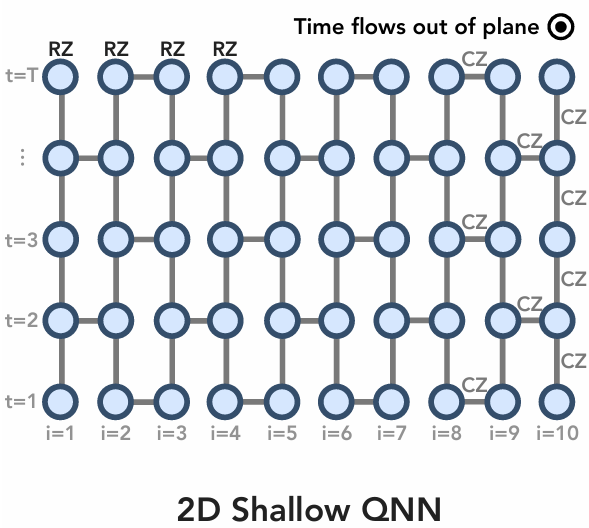
\includegraphics[width=0.98\linewidth,height=0.58\textheight,keepaspectratio]{2D Shallow QNN.png}

    \vspace{0.35em}
    {\scriptsize 2D shallow QNN architecture used by IDQNN.}

    \column{0.50\textwidth}
    \centering
    \resizebox{0.98\linewidth}{!}{%
    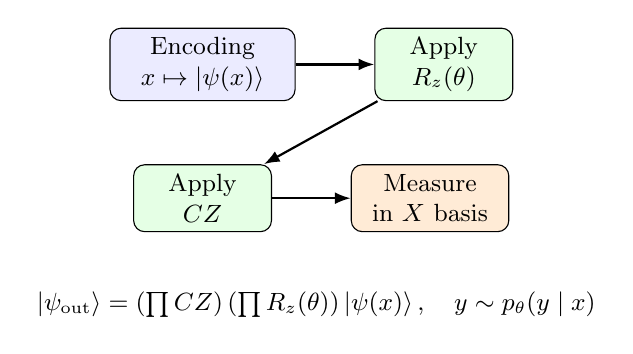
\begin{tikzpicture}[
      font=\small,
      node distance=8mm and 10mm,
      box/.style={draw, rounded corners, minimum width=2.35cm, minimum height=0.85cm, align=center, fill=blue!8},
      op/.style={draw, rounded corners, minimum width=1.75cm, minimum height=0.85cm, align=center, fill=green!10},
      meas/.style={draw, rounded corners, minimum width=2.0cm, minimum height=0.85cm, align=center, fill=orange!16},
      arrow/.style={-{Latex[length=2mm]}, thick}
    ]
      % 2x2 layout
      \node[box] (enc) {Encoding\\$x\mapsto \ket{\psi(x)}$};
      \node[op, right=of enc] (rz) {Apply\\$R_z(\theta)$};
      \node[op, below=of enc] (cz) {Apply\\$CZ$};
      \node[meas, right=of cz] (mx) {Measure\\in $X$ basis};

      % flow: top row -> down -> bottom row
      \draw[arrow] (enc) -- (rz);
      \draw[arrow] (rz) -- (cz);
      \draw[arrow] (cz) -- (mx);

      \node[align=center] at ($(cz)!0.5!(mx)+(0,-1.35)$)
      {$\ket{\psi_{\mathrm{out}}}=\left(\prod CZ\right)\left(\prod R_z(\theta)\right)\ket{\psi(x)},\quad y\sim p_\theta(y\mid x)$};
    \end{tikzpicture}%
    }
  \end{columns}

  \vspace{0.35em}
  \begin{block}{Input-state encoding rule}
    {\footnotesize Qubit $i$ is initialized from
    $\{|0\rangle, |+\rangle=\tfrac{1}{\sqrt{2}}(|0\rangle+|1\rangle)\}$ according to bit $x_i$:
    $0\mapsto|+\rangle,\;1\mapsto|0\rangle$.}
  \end{block}
\end{frame}

\begin{frame}{Learning Algorithm: parameters Estimation}
  \small
 
  {\bfseries Learning stratage}
  \begin{itemize}
    \item For each parameter at position $(i,j)$, filter samples satisfying:
    \[
      x_{i,j}=0,\qquad x_{\mathcal N(i,j)}=1,
    \]
    where $\mathcal N(i,j)$ denotes positions connected via CZ gates.
    \item Compute the parameter estimate from the filtered samples.
  \end{itemize}

  \[
    \hat\theta_{i,j}=\arccos\!\left(1-\frac{2}{N_{\mathrm{sp}}}\sum_{t=1}^{N_{\mathrm{sp}}}y^{(i,j)}_{(t)}\right).
  \]

\end{frame}

\begin{frame}{Advantage in artical}
  \begin{block}{Dataset generation}
    Using ideal parameters $\theta^*$ and IDQNN circuit, generate dataset:
    \[
      \mathcal{D} = \{(x_i, y_i)\}_{i=1}^{N_{\mathrm{sample}}}.
    \]
  \end{block}
  \vspace{1.35em}
  Quantum models can learn underlying distributions over $\mathcal{D}$ which classical models struggle with.
\end{frame}



\section{MNIST Training Setup}

\begin{frame}{New Question: MNIST Training Performance}
  \begin{block}{Question}
    How well do DQNN/IDQNN train on a practical handwritten-digit task?
  \end{block}
  \vspace{1.8em}
  \begin{itemize}
    \setlength{\itemsep}{6pt}
    \item MNIST training set: 60,000 samples; test set: 10,000 samples.
    \item Original image size: $28\times28=784$ grayscale pixels, normalized to $[0,1]$.
    \item We construct a learning dataset $\mathcal D_{\mathrm{MNIST}}=\{(x_i,y_i)\}_{i=1}^{60000}$ .
  \end{itemize}

\end{frame}

\begin{frame}{Runtime: DQNN vs IDQNN}
  \begin{alertblock}{Key practical point}
    DQNN and IDQNN generate the same distribution, but runtime differs significantly in practice.
  \end{alertblock}
  \vspace{0.4em}
  \small
  \begin{itemize}
    \item DQNN uses only $m$ qubits; IDQNN uses $n_1\times m$ qubits in the shallow representation.
    \item Measured sampling runtime in our implementation:
  \end{itemize}

  \vspace{0.4em}
  \centering
  \begin{tabular}{lcc}
\toprule
Model & input $x$ size & Sampling time (single run) \\
\midrule
DQNN & $10\times10$ ($n=100$) & $1.8\,$s \\
IDQNN & $5\times5$ ($n=25$) & $44.019\,$s \\
\bottomrule
\end{tabular}

\end{frame}

\begin{frame}{Preprocessing: Resize to 10\texorpdfstring{$\times$}{x}10 for Input $x$}
  \begin{itemize}
    \item We reshape each MNIST image to a $10\times10$ grayscale image.
    \item The resulting 100-pixel vector is mapped to the input bitstring $x$.
  \end{itemize}

  \centering
  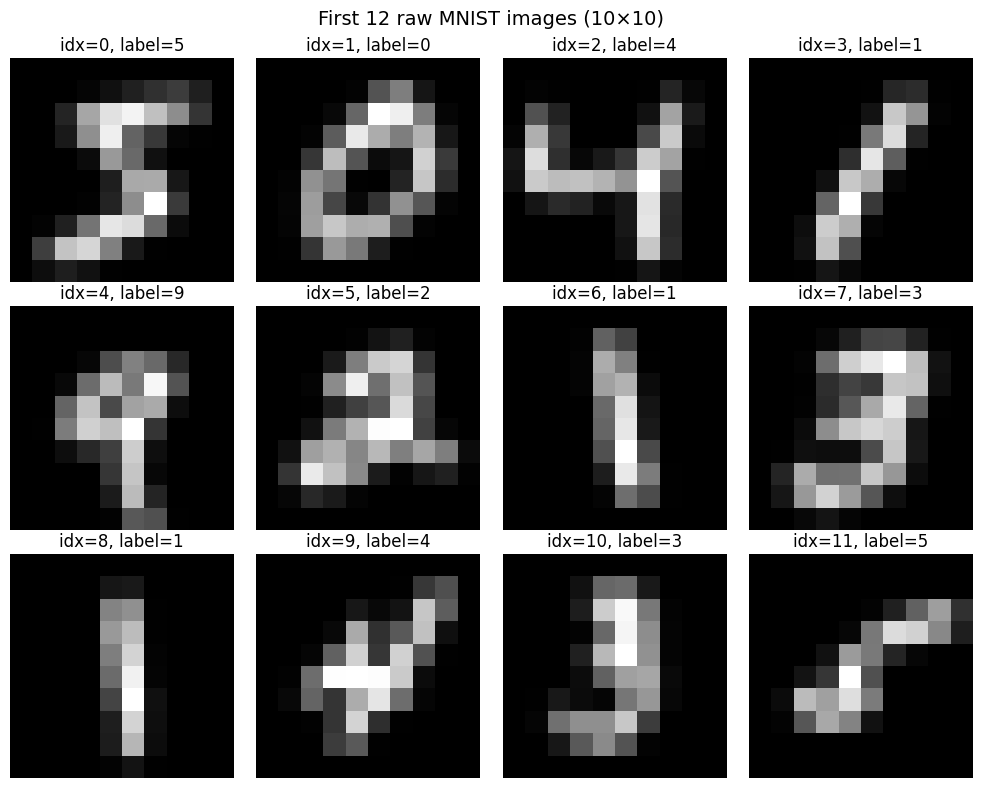
\includegraphics[width=0.96\linewidth,height=0.68\textheight,keepaspectratio]{First 12 raw MNIST images (10×10).png}
\end{frame}

\begin{frame}{Binarization and Threshold Choice}
  \begin{columns}[c,onlytextwidth]
    \column{0.48\textwidth}
    \centering
    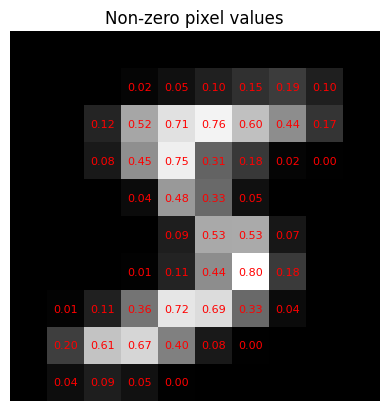
\includegraphics[width=0.98\linewidth,height=0.70\textheight,keepaspectratio]{Non_0_pixel_values.png}

    \column{0.48\textwidth}
    \textbf{Data Binarization:}
    \centering
    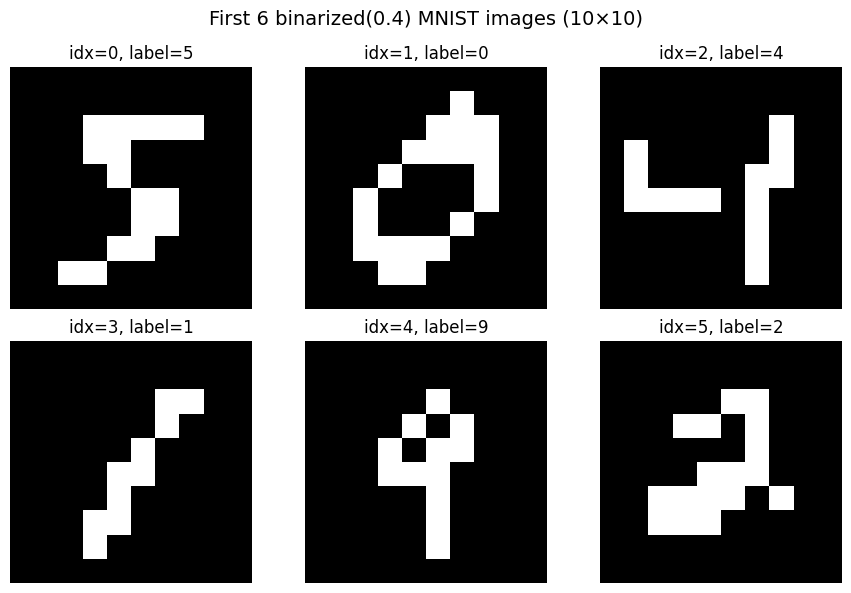
\includegraphics[width=0.98\linewidth,height=0.70\textheight,keepaspectratio]{First 6 binarized MNIST images (10×10).png}
  Gain the train input data $\{x_i\}$.
  \end{columns}
\end{frame}

\begin{frame}{Label-Bitstring Encoding for $y$ (0--9)}
  \small
  \centering
  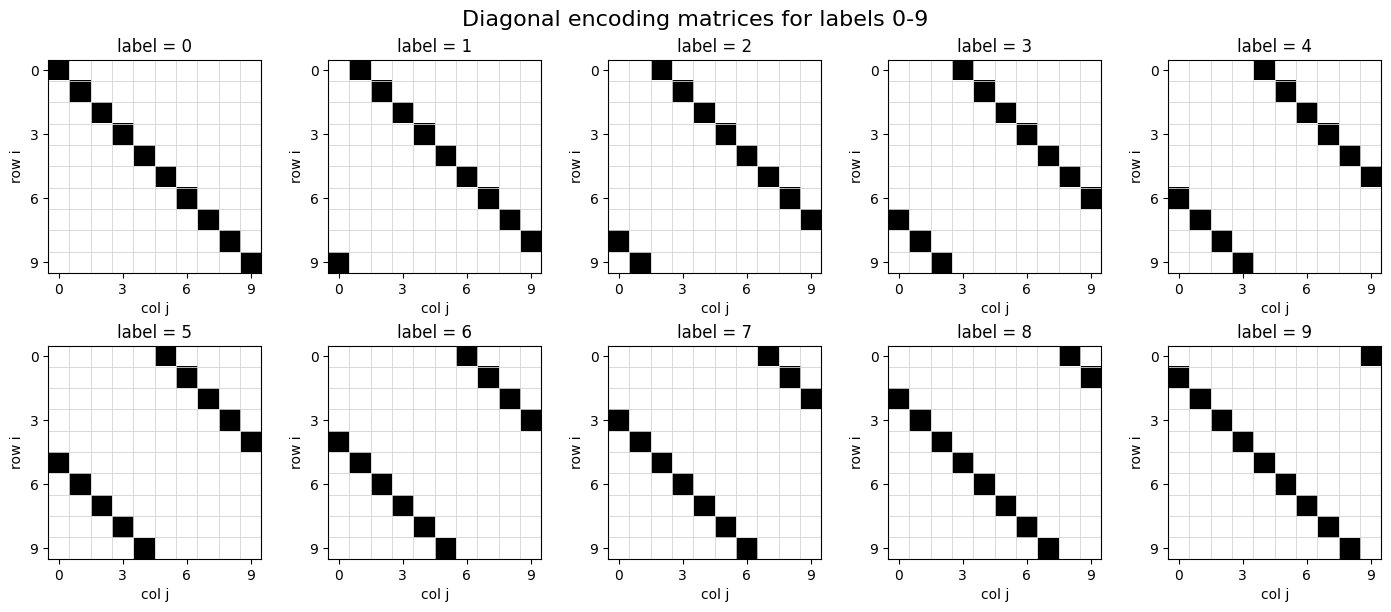
\includegraphics[width=0.98\linewidth,height=0.78\textheight,keepaspectratio]{encoding1.png}

  \vspace{0.35em}
  {\footnotesize Encoding pattern for digit labels $0$--$9$.}
  Gain the datasets $\{x_i,y_i\}$, both $x$ and $y$ are 100-bit strings.
\end{frame}

\section{MNIST Estimation and Generation}

\begin{frame}{Filter-Sample Statistics for Parameter Estimation}
  \begin{columns}[c,onlytextwidth]
    \column{0.58\textwidth}
    \centering
    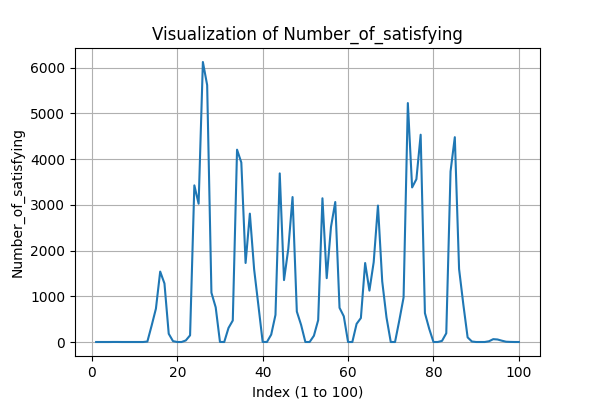
\includegraphics[width=0.98\linewidth,height=0.64\textheight,keepaspectratio]{Visualization_of_Number_of_satisfying.png}

    \column{0.40\textwidth}
    \scriptsize
    \begin{block}{Valid Sample Statistics：}
      \begin{itemize}
        \item We first count valid filter samples for each parameter position.
        \item Skipped bits ($N_{\mathrm{sp}}=0$): 21.
        \item Indices (0-based): $[0,1,2,3,\ldots,29,\ldots,50,\ldots,99]$.
      \end{itemize}
    \end{block}
    Parameters with no valid samples are set to 0.
  \end{columns}
\end{frame}

\begin{frame}{Generation on Test Set with Learned Parameters}
  \small
  \begin{itemize}
    \item After estimating $\theta$, we generate $y$ on test inputs.
    \item Example: for test index 99, we sampled 1000 generated outputs and averaged the generated bits.
    \item The averaged generated pattern is compared with the true encoded label.
  \end{itemize}

  \vspace{0.2em}
  \begin{columns}[c,onlytextwidth]
    \column{0.30\textwidth}
    \centering
    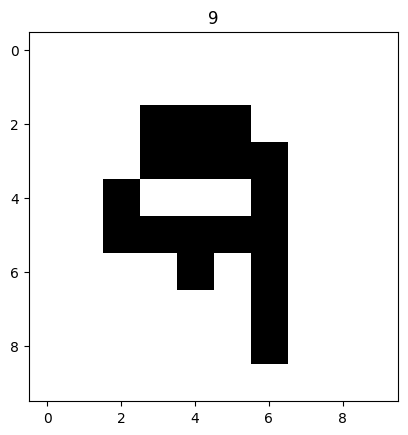
\includegraphics[width=0.98\linewidth,height=0.42\textheight,keepaspectratio]{test_bitstring_99.png}

    \column{0.68\textwidth}
    \centering
    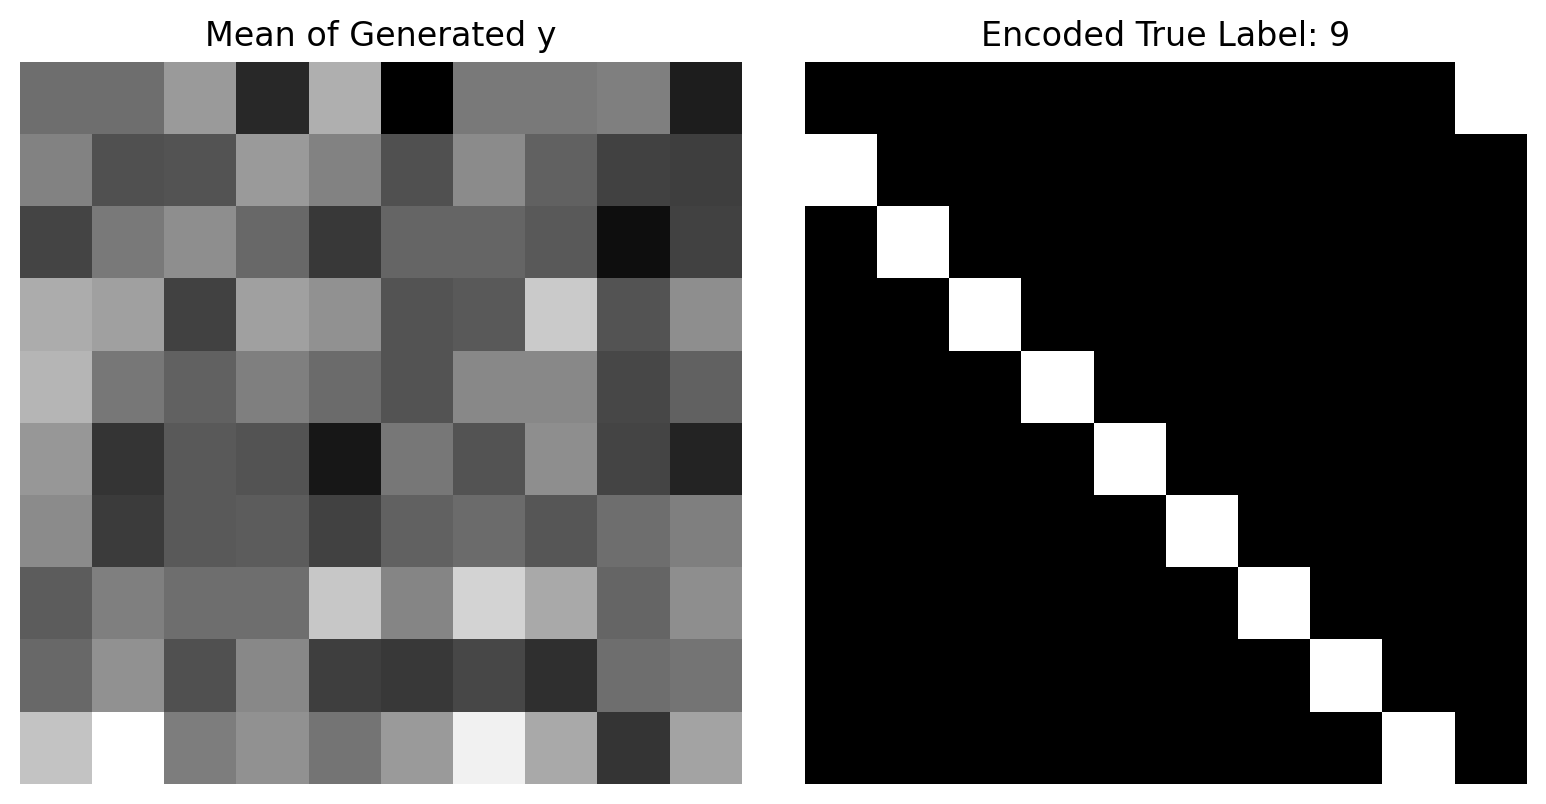
\includegraphics[width=0.98\linewidth,height=0.42\textheight,keepaspectratio]{mean_vs_encoded_n1_10_m_10_seed_42_nNumber_1000_testIdx_99_trueLabel_9_bitstring_1111111111111111111111100011111110000111110111011111000001111111010111111111011111111101111111111111.png}
  \end{columns}
\end{frame}

% \begin{frame}{Conclusions}
%   \begin{itemize}
%     \item We extended the inference+learning pipeline from synthetic data to MNIST-derived bitstring data.
%     \item DQNN is significantly faster than IDQNN in our sampling tests, while preserving equivalent target distribution.
%     \item Binarization threshold and filter-sample coverage strongly affect parameter estimation quality.
%     \item Preliminary test-set generation shows meaningful alignment with encoded target labels.
%   \end{itemize}

%   \vspace{0.4em}
%   \begin{block}{Next steps}
%     Improve sparse-filter handling, compare threshold strategies systematically, and benchmark against classical baselines on the same encoded task.
%   \end{block}
% \end{frame}

\end{document}
